
I focus on the impact that civilian exclusion orders following Executive Order 9066
had on the migration choices that the internees faced after their release from the camps.
To model the unexpected shock to the internees lifetime career plans and subsequent migration decisions,
I apply the model of individual migration choices developed by \cite{kennanEffectExpectedIncome2011} 
to the migration choices I observe among Japanese and Chinese Americans from 1935 to 1950.

Due to the limits of the historical data available to me for this time period,
I make several simplifications to the choices faced by potential migrants.
Specifically, I follow \citeauthor{kennanEffectExpectedIncome2011} by only considering the partial equilibrium effect
of permanent wage levels across different counties on workers' migration choices.
This leaves out the influence of fixed assts like farms, houses, and small businesses
which cannot be easily brought along when their owners move away (either voluntarily or by evacuation order).

The benefits of using this model are that because it includes forward-looking decision making of workers,
I can treat the unexpected nature of the evacuation and internment orders as a shock to the moving costs faced by 
internees between their location choice in 1940 (prior to internment) and 1950.

\subsection{DAG}

\begin{center}
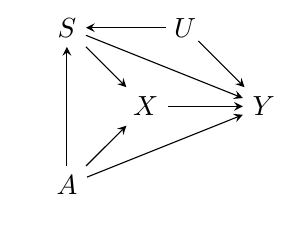
\begin{tikzpicture}
  \tikzset{
      > = stealth,
      every node/.append style = {
      },
      every path/.append style = {
          arrows = ->,
      },
      hidden/.style = {
          shape = circle,
          inner sep = 1pt
      }
  }
  \tikz{
      \node (a) at (0,0) {$A$};
      \node (s) at (0,2) {$S$};
      \node (x) at (1,1) {$X$};
      \node (y) at (2.5,1) {$Y$};
      \node[hidden] (u) at (1.5,2) {$U$};
      \path (a) edge (s);
      \path (a) edge (x);
      \path (a) edge (y);
      \path (s) edge (x);
      \path (s) edge (y);
      \path (x) edge (y);
      \path (u) edge (s);
      \path (u) edge (y);
  }
   
\end{tikzpicture}
\end{center}

\subsection{Worker Preference for Location}

A worker in this model chooses to move between $J$ locations to maximize their total discounted lifetime utility.

The flow utility to this worker of choosing to work in location $j$ is decomposed as
$$\tilde{u}_h(x,h))=u_h(x,j) + \xi_j$$
where $u_h(x,j)$ includes all components of the worker's preference for $j$ which are observable to me as the researcher,
and $\xi_j$ represents the worker's immediate value of all elements of location $j$ which are unobservable.

The observable portion of the flow utility is defined as follows for a worker who's home location is $h$:
\begin{equation}
u_h(x,j) = \alpha_0 w(\ell^0,\omega) + \alpha^H \mathbb{I}(\ell^0=h) + \sum_{k=1}^{K}\alpha_kY_k(\ell^0)
+ \xi(\ell^0,\omega) - \Delta_\tau(x,j)
\end{equation}
where
$w(\ell^0,\omega)$ is the wage income in the current location $\ell^0$,
and $\mathbb{I}(\ell^0=h)$ is the indicator which is equal to 1 if the current location is the worker's home location and 0 otherwise.
This flow utility conditions on a vector of $K$ observable amenities of each location 
which all workers have common preferences for represented by $alpha_k$.
$\Delta_\tau(x,j)$ is the moving cost from location $\ell^0$ to location $j$.

\subsubsection{Moving Costs}

The subjective moving costs faced by a worker considering a move from their current location $\ell^0$ to $j$
(which could either be a new location, or the same location, i.e., no move),
is modelled as:
\begin{equation}
  \Delta_\tau(x,j) = \mathbb{I}(j\neq\ell^0) 
  \left[ 
    \gamma_{0\tau} + \gamma_1 D(\ell^0, j) - \gamma_2 \mathbb{I}(j\in\mathbb{A}(\ell^0))
    - \gamma_3 \mathbb{I}(j=\ell^{-1}) + \gamma_4a - \gamma_5 n_j
  \right]
\end{equation}
where they pay zero moving cost if they choose not to move ($j=\ell^0$).
If the worker moves to a new location, they pay a fixed cost $\gamma_{0\tau}$ 
as well as a variable cost which depends on the distance to the new county ($D(\ell^0, j)$).
The fixed cost potentially depends on their type $\tau$ to represent the possibility that there are certain types of people who are always stayers.


\begin{equation}
V(x,\xi) = max_j(v(x,j)+\xi_j)
\end{equation}
where
\begin{equation}
v(x,j) = u(x,j) + \beta \sum_{x'}p(x' | x,j) \bar{v}(x')
\end{equation}
and
\begin{equation}
\bar{v}(x) = \mathbb{E}_{\xi} [V(x,\xi)]
\end{equation}

The expected benefit you will get in the future from location $j$ is the expected value over all of the potential moves you could make, weighted by how likely each potential move would be based on your preference shock $\xi_j$ .